Nachdem die aktuelle Situation analysiert wurde, wurde mit der Planung der Applikation begonnen. Die folgenden Abschnitte Orientieren sich anhand der vorgaben des Pflichtenhefts.\todo LINK PLFICHTENHEFT

\subsection{Applikationsart}

Wie bereits unter \sct{sec:Einführung-Definitionsphase:Projektziel}{Projektziel} genannt, soll die Applikation als Webapplikation entwickelt werden. Ein Grund dafür ist, dass man die Applikation so in der Zukunft
vergleichsweise einfach aktualisieren kann. Der Technologie Stack \gl{MERN} wird für die Erstellung der Softwarelösung gewählt, weil dieser generell etabliert und bereits in dem Software Development Team verwendet und in diverse Projekten bereits umgesetzt wird. Dadurch kann gegebenenfalls vom Know-How anderer Personen im Team profitiert werden. So wird die Serverapplikation mit \gl{express} auf der Laufzeitumgebung \gl{nodejs} und \gl{SPA} mit \gl{React} entwickelt und \gl{MongoDB} zur Speicherung von Daten verwendet werden.

\subsection{Applikationsarchitektur}
\label{sec:Planungsphase:Applikationsarchitektur}

Die Softwarelösung wird in zwei Teilapplikationen entwickelt: \sct{sec:Planungsphase:Frontend}{Frontend} und \sct{sec:Planungsphase:Backend}{Backend}. Eine Backend Applikation ist Notwenig da sich bereits auf eine \gl{SPA} festgelegt wurde. Da eine \gl{SPA} nicht sicher mit Daten interagieren kann.

\subsubsection{Frontend}
\label{sec:Planungsphase:Frontend}

Das Frontend wird durch eine \gl{SPA} repräsentiert. Eine \gl{SPA} ist eine Applikation, die vollständig im Browser ausgeführt wird.  Im Gegensatz zu üblichen Server-Side Webanwendungen wird nicht bei jeder Interaktion mit dem Server \gl{HTML} zurückgegeben und vom Browser dargestellt.Statt dessen wird die Interaktion durch browserseitiges \gl{JS} ausgeführt.
So wird beispielsweise bei der Erstellung einer \gl{RA} mithilfe des Chatbots, eine Anfrage an das Backend gestellt, welches dann eine passende Frage zurückgibt. Diese Informationen werden anschließend vom Frontend verarbeitet und angezeigt.

\subsubsection{Backend}
\label{sec:Planungsphase:Backend}

Das Backend läuft auf dem Server und und übernimmt die gesamte Datenverwaltung und Businesslogik. Mit \gl{mongoose} kann das Backend dann auf die gespeicherten Daten der \gl{MongoDB} zugreifen.
Da die beiden Teilapplikationen miteinander kommunizieren müssen stellt das Backend eine \gl{REST}-\gl{API} zur Verfügung. Über diese kann dann das Frontend Informationen senden. Um so z.B. \glp{RA} einreichen zu können.
Das Backend wird auf Basis der \gl{MSC}-Architektur entwickelt. Dabei werden die Komponenten nach Typ unterteilt. In der \gl{MSC}-Architektur gibt es folgende Komponententypen:

\begin{enumerate}
  \item \textbf{M}odel\\
  Das Model beschreibt die zu speichernden Daten im Rahmen einer einzelnen Entität. So werden im Model die klassischen CRUD-Operationen durchgeführt. Wie das Kreieren einer \gl{RA}.
  \item \textbf{S}ervice\\
  Im Service findet die gesamte Logik statt. Services sind die einzigen Komponenten der Applikation, die mit Models interagieren. Sie bieten die Möglichkeit, die CRUD-, und gegebenenfalls noch weitere, Operationen auszuführen. Wie die Hintergrundberechnungen von Pauschalen.
  \item \textbf{C}ontroller\\
  Controller sind die Komponenten, die die tatsächliche Interaktion mit der Außenwelt, also dem \gl{HTTP}-Client übernehmen. Sie interagieren mit den Services, um die Anfragen des Clients auszuführen. Der Punkt, an dem die Daten vom Frontend an die Services zur Verarbeitung gesendet werden.
\end{enumerate}

Neben diesen Hauptkomponenten gibt es die folgenden Komponenten:

\begin{itemize}
  \item Middleware\\
Neben den vorinstallierten oder heruntergeladenen Middlewares können auch eigene erstellt werden. Im konkreten Fall wird eine Middleware verwendet, die den Zugriff auf bestimmte Bereiche der Applikation einschränkt. Dadurch wird eine Anfrage bereits vor dem Eintreffen im Controller beantwortet, falls bestimmte Anforderungen nicht erfüllt sind. So können z.B. nur Benutzer mit der Prüfer Rolle die Prüfungsansicht einsehen.
  \item Tests\\
  Die Tests dienen dazu, die einzelnen Komponenten auf verschiedene erwartete Ergebnisse hin zu überprüfen. Dabei werden die kritischen Berechnungsfunktionen auf ihr vorgesehenes Verhalten geprüft.
\end{itemize}

Eine Kernkomponente des Backends ist die Logik des Chatbots. Hierfür werden Endpoints bereitgestellt, die über das Frontend erreicht werden können. Bei jeder Benutzerantwort erhält das Backend eine Anfrage, die die ursprüngliche Frage und die dazugehörige Antwort enthält. Das Backend prüft nun, welche Folgefrage anhand der gegebenen Antwort zu dieser ursprünglichen Frage zurück an das Frontend gegeben wird. Parallel dazu wird die Antwort gespeichert.

\subsection{Modelle und Datenstruktur}
\label{sec:Planungsphase:ModelleDatenstruktur}

Die Anforderungen machen deutlich, dass mehrere Modelle und Datenstrukturen erforderlich sind. So wird ein Modell für die Länder und deren Pauschalen benötigt, die Reisekostenabrechnung, die sich aus dem Chatverlauf ergibt, sowie Grundinformationen und Dienstreisen welche die Informationen aus dem Chat verarbeiteten, sowie ein Modell, das einige Berechnungsgrundlagen speichert. Außerdem wird ein Benutzermodell benötigt, um die jeweiligen Vorgesetzten zu speichern und ein Modell welches die Fragen für den Chatbot abspeichert.
Die Chatverläufe müssen ebenfalls gespeichert werden, um eine spätere Anpassung der \gl{RA} zu ermöglichen durch.

\subsubsection{Chatbot Datenstruktur und Logik}
\label{sec:ModelleDatenstruktur:ChatbotDatenstrukturLogik}

Die Struktur wurde so gestaltet, dass das Backend schnell und einfach die nächste Folgefrage ermitteln kann. Hierbei verweist die Ausgangsfrage auf die Folgefragen.
Diese Struktur bietet Vorteile in Bezug auf die Wartbarkeit, da bei Anpassungen an den Fragen keine Änderungen am Quellcode notwendig sind.

Die Chatbot-Fragen sind in der Datenbank wie folgt gespeichert:\\
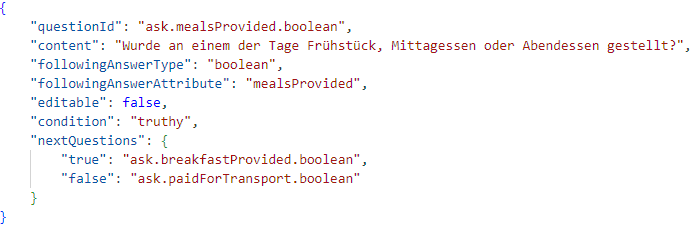
\includegraphics[width=1\textwidth]{fragestruktur.png}

Um Folgefragen zu ermitteln, wird das Objekt \verb|nextQuestions| in Verbindung mit dem Attribut \verb|condition| verwendet, um eine If-Abfrage zu bilden. Dadurch wird geprüft, ob die Antwort auf diese Frage \textit{true} oder \textit{false} ist, und basierend auf dem Ergebnis wird die entsprechende Frage aus \verb|nextQuestions| an das Frontend zurückgegeben.

Bei Fragen die keine \verb|condition| haben, also keine Abzweigungen, enthält das \verb|nextQuestions| Objekt ein Attribut namens \verb|default| diese wird dann dem Frontend zurückgegeben.

Im Anhang ist eine visualisierte Form der Fragenabfolge des Chatbots in Form eines \sct{sec:Anhang:DecisionTree}{Decision Trees} zu finden.  

\subsection{Feststellung der Benutzerberechtigungen}
\label{sec:Planungsphase:Benutzerberechtigungen}

Das unter \sct{sec:Analysephase:Benutzerklassifizierung}{Benutzerklassifizierung} beschriebene Benutzerkonzept sieht drei Benutzerklassen vor. Es wird davon ausgegangen, dass jeder Benutzer, der sich an der Anwendung bzw. am \gl{IDP} anmeldet, zunächst ein Regulärer Benutzer ist. Anschließend wird geprüft, ob ein Benutzer über eine Rolle verfügt, die ihm über den \gl{IDP} zugewiesen wurde.
